\section{Are you still friends with any of your friends from high school? How have they changed since then?}
Sorry to say I am not in contact with friends from high school.
However I do keep in contact with two women with whom I shared an apartment as a young adult.
Sandi Bontrager Harnish and Rose Brubaker Kennel.
We shared an apartment from fall of 1977 to summer of 1979.
\begin{figure}
\centering
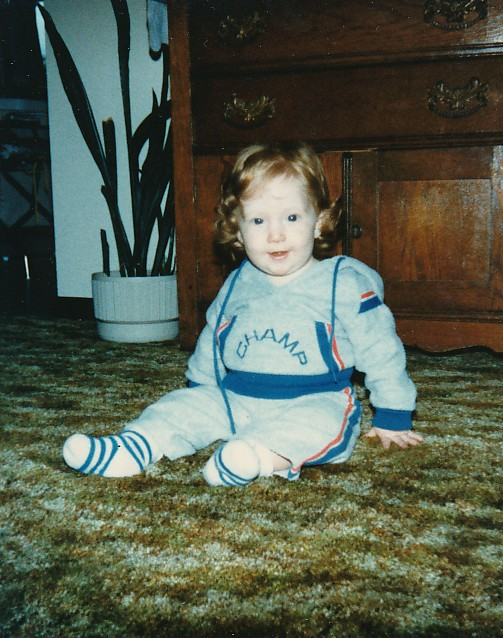
\includegraphics[width=0.9\textwidth]{childhood/12.jpg}
\caption{
Lois, Rose and Sandi
}
\end{figure}

Sandi grew up in northern Indiana and married a Lancaster County farmer, Martin Harnish.
She lives a few miles from the farm where I grew up.
You might say that we switched places since I now live in northern Indiana some miles from where she grew up.

Sandi and Martin have two children.
The oldest, Amanda is a few weeks older than Tim.
Sandi and I traded baby due dates and Amanda was born mid-April while Tim waited until early May to be born.
While we went through the pregnancy at the same time I expected to have my baby first but the babies did not agree and made the trade.
\begin{figure}
\centering
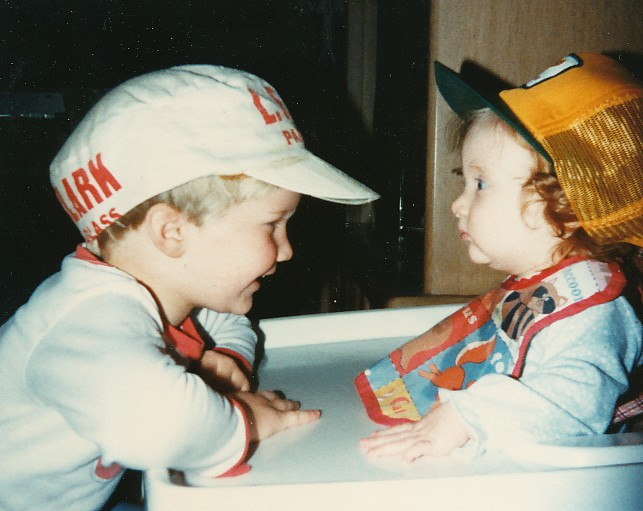
\includegraphics[width=0.5\textwidth]{childhood/13.jpg}
\caption{
Amanda and Tim
}
\end{figure}
Daniel, their second child was born the same year as Abby.
So while our children were small Sandi and I saw each other at mother's groups.

Rose married John's friend, Chris Kennel.
She taught school for many years and then pre-school.
Rose and Chris have two children, Eric and Carmen.
Eric and Tim are the same age and Carmen was between Abby and Jonathan.
We have memories of a weekend spent with them at their cabin in the Pennsylvania Mountains.
\begin{figure}
\centering
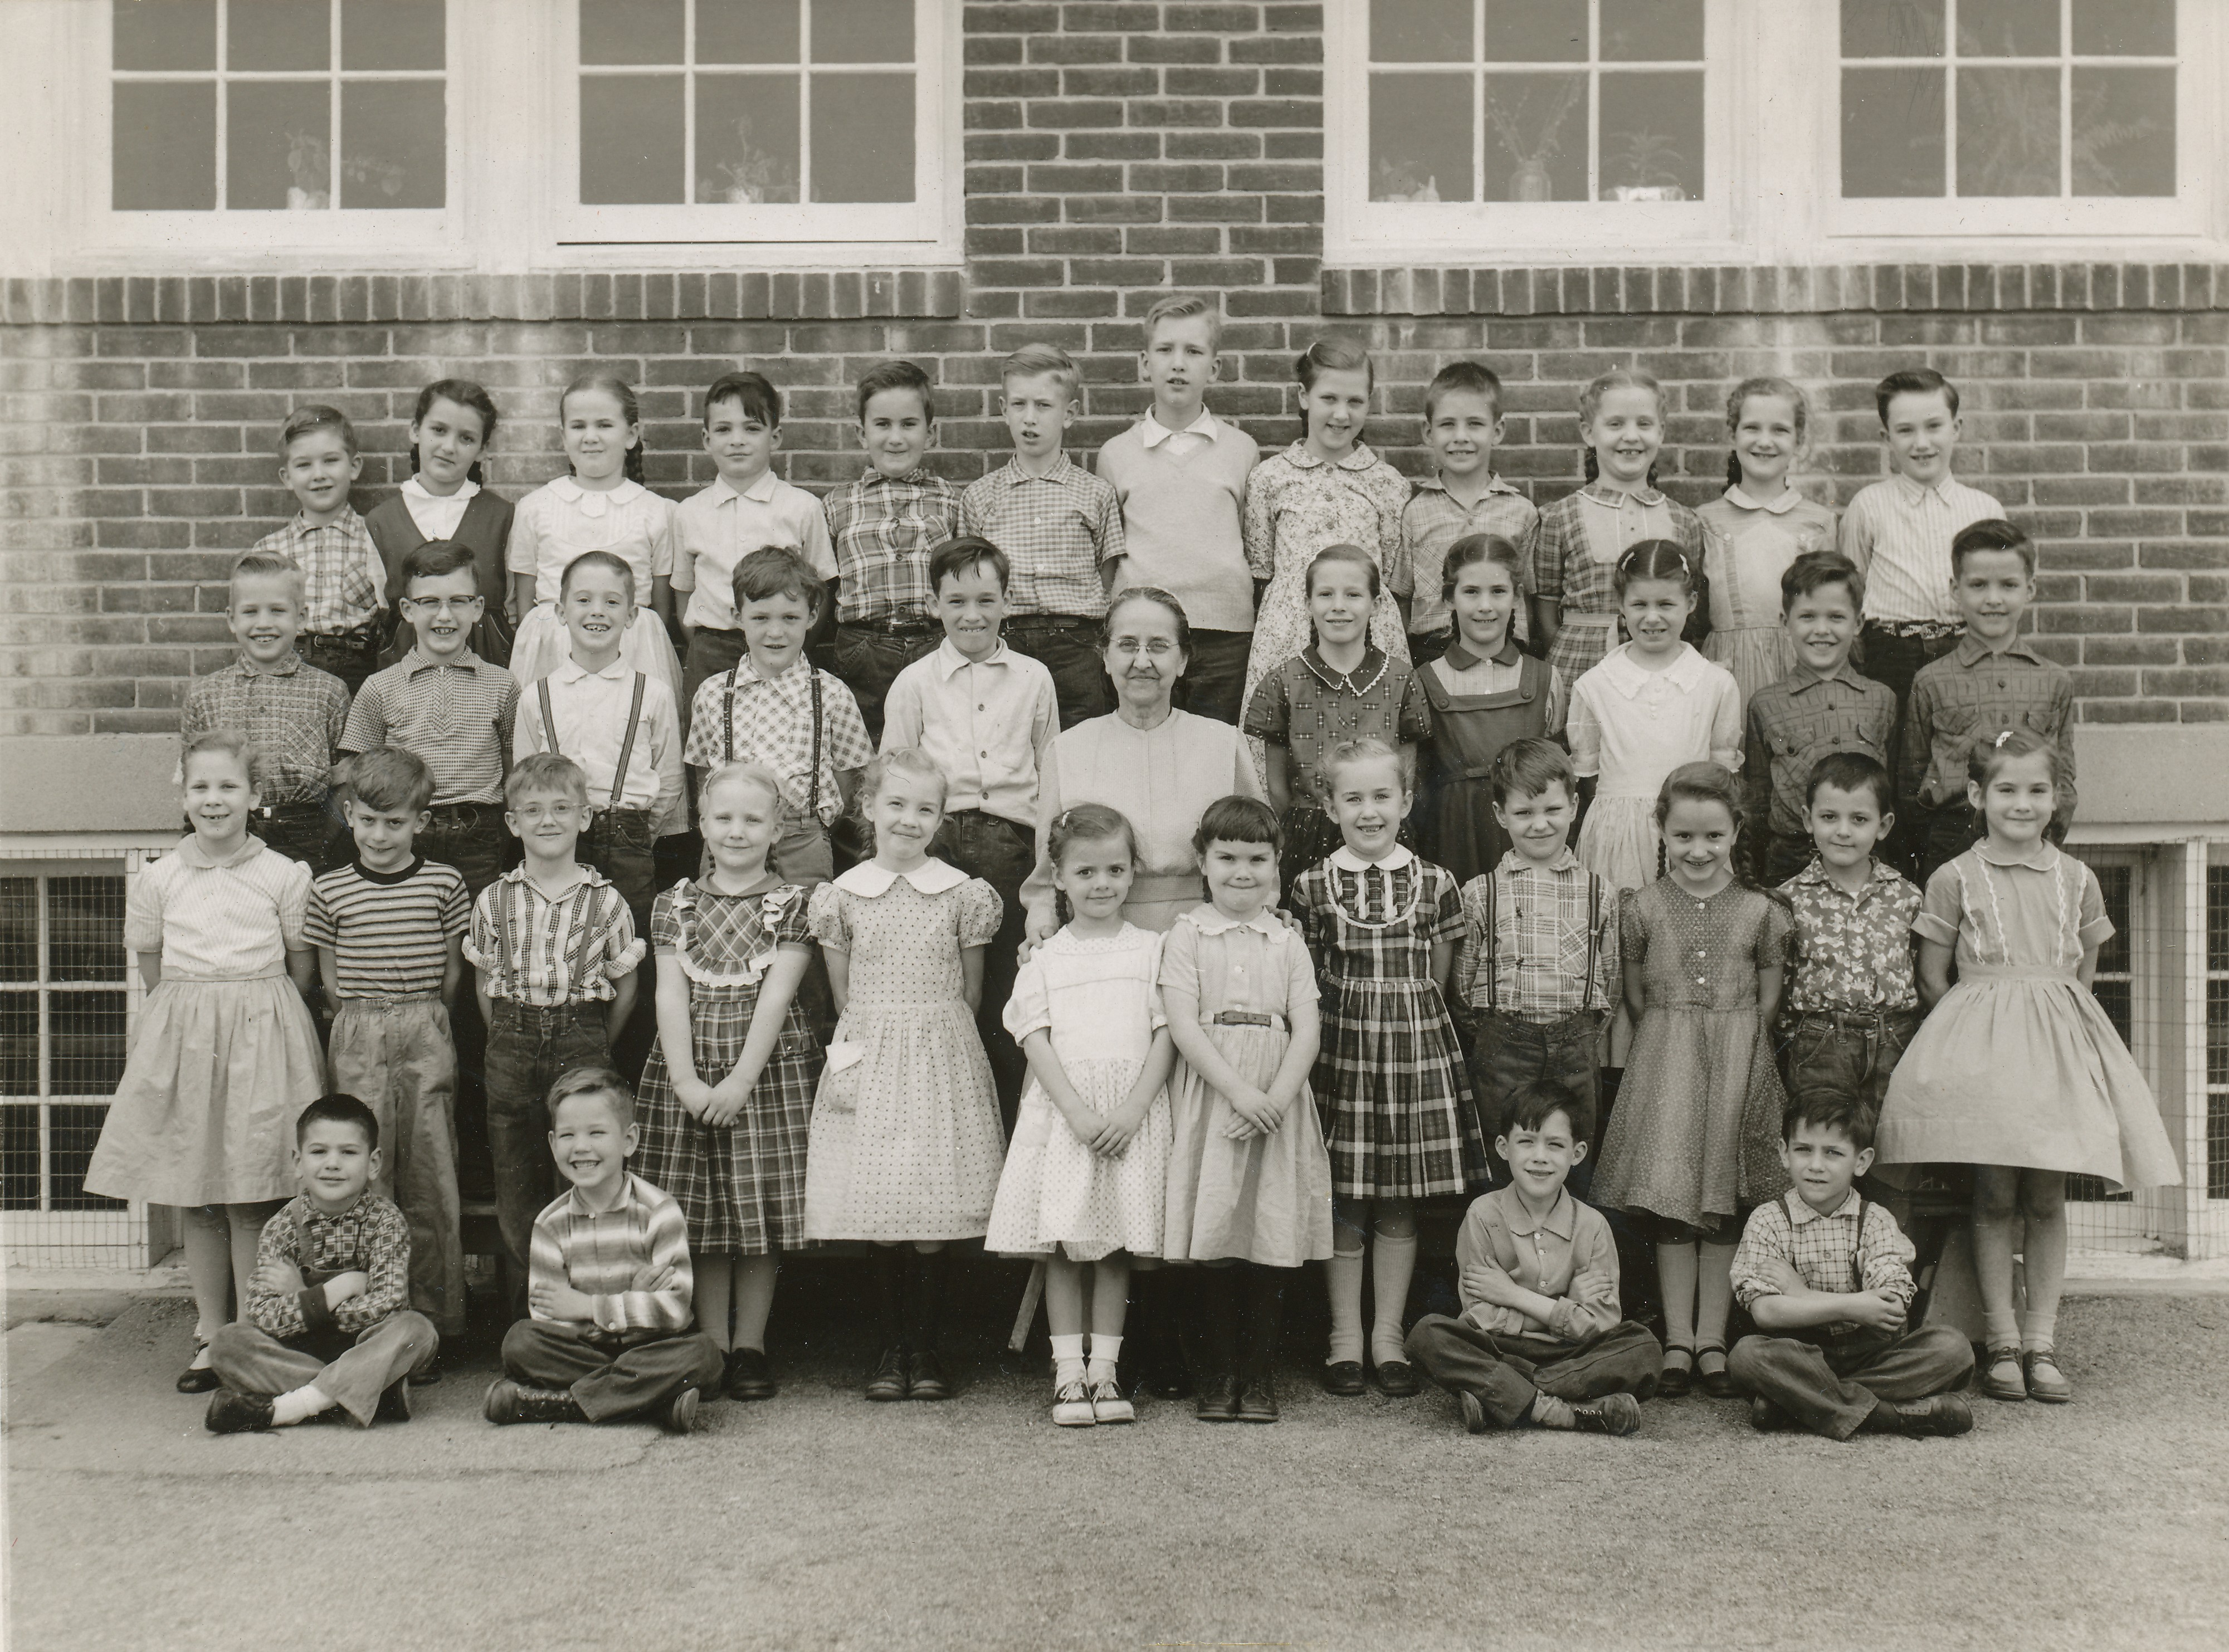
\includegraphics[width=0.9\textwidth]{childhood/14.jpg}
\caption{
Eric and Tim
}
\end{figure}
We enjoy connecting with these couples when we spend time in Lancaster County and time permits.
They have both hosted us as well.







